\documentclass{beamer}
\usepackage{graphicx}
\usepackage{amsmath}
\usepackage{amssymb}
\usepackage{wrapfig}

\title[Mechanics of Materials]{Mechanics of Materials}
\subtitle{Week 3}
\author{Lecturer: Viggo K. Hansen}
\institute{Faculty of Engineering, Chulalongkorn University}
\date{Academic Year: 2024 \\ Semester: Second}

\begin{document}

% Title Slide
\frame{\titlepage}

% Slide: Overview
\begin{frame}{Overview}
    \tableofcontents
\end{frame}

% Section: Deformation of Axially Loaded Members
\section{Deformation of Axially Loaded Members}
\begin{frame}{Deformation of Axially Loaded Members}
    \begin{minipage}[t]{0.4\textwidth}
        \begin{itemize}
            \item Axially loaded members deform under applied axial forces.
            \item \textbf{Normal stress ($\sigma$):} $\sigma = \frac{P}{A}$, where $P$ is the axial force and $A$ is the cross-sectional area.
            \item \textbf{Axial deformation ($\delta$):} $\delta = \frac{PL}{AE}$, where $L$ is the length of the member, $E$ is the modulus of elasticity.
            \item Assumptions include small deformations and linear elastic behavior (Hooke's Law).
        \end{itemize}
    \end{minipage}
    \hfill
    \begin{minipage}[t]{0.55\textwidth}
        \vspace{0pt}
        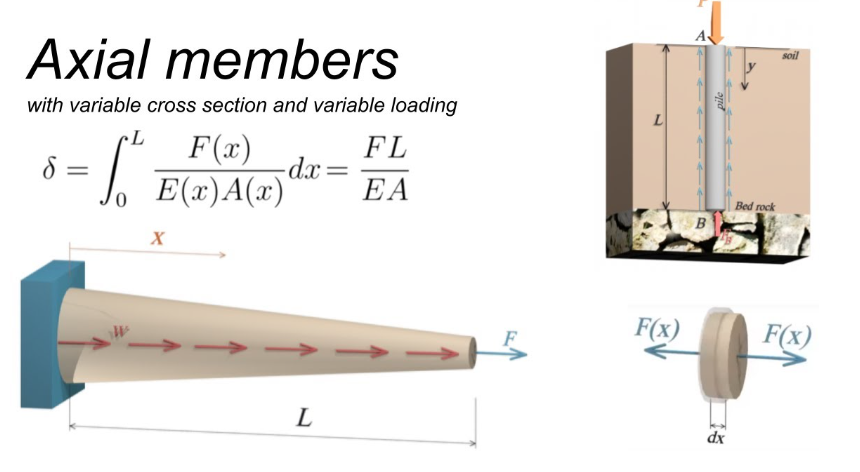
\includegraphics[width=\textwidth]{Axial_Deformation.png}
    \end{minipage}
\end{frame}

% Section: Thermal Stress
\section{Thermal Stress}
\begin{frame}{Thermal Stress}
    \textbf{Definition:}
    Stress induced in a material due to temperature changes when expansion or contraction is restrained.
    \vspace{0.5cm}

    \textbf{Key Formula:}
    \[ \sigma = E \alpha \Delta T \]
    Where:
    \begin{itemize}
        \item $E$: Modulus of elasticity
        \item $\alpha$: Coefficient of thermal expansion
        \item $\Delta T$: Change in temperature
    \end{itemize}
\end{frame}

% Section: Tension Test and Stress-Strain Behavior
\section{Tension Test and Stress-Strain Behavior}
\begin{frame}{Tension Test}
    \textbf{Tension Test:}
    \begin{itemize}
        \item Evaluates material strength and behavior under axial tension.
        \item Generates a plot of normal stress ($\sigma$) versus normal strain ($\varepsilon$).
    \end{itemize}
    \vspace{0.5cm}
    \textbf{Key Regions of the Stress-Strain Curve:}
    \begin{minipage}[t]{0.45\textwidth}
        \begin{itemize}
            \item \textbf{Elastic Region:} Linear relationship where $\sigma = E\varepsilon$.
            \item \textbf{Yield Point:} Transition from elastic to plastic deformation.
            \item \textbf{Strain Hardening:} Stress increases with strain post-yield.
            \item \textbf{Necking and Fracture:} Material begins to neck, leading to failure.
        \end{itemize}
    \end{minipage}
    \hfill
    \begin{minipage}[t]{0.5\textwidth}
        \vspace{0pt}
        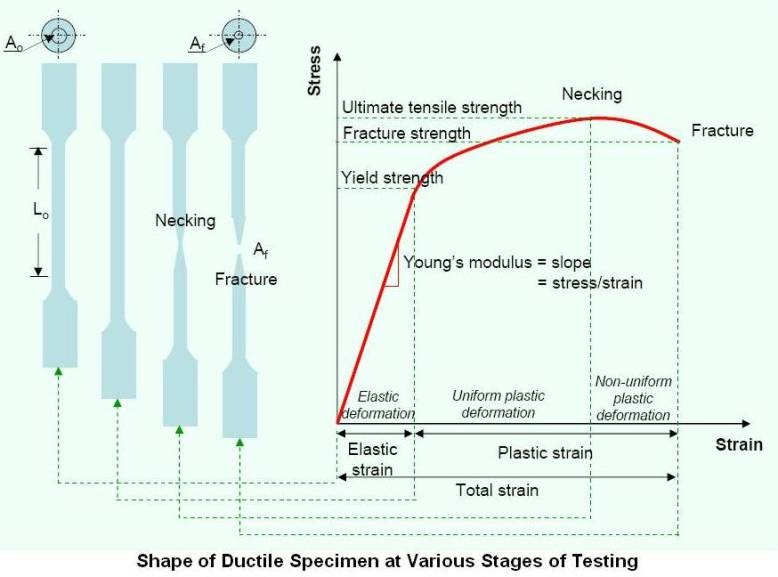
\includegraphics[width=\textwidth]{Tension_Test.jpg}
    \end{minipage}
\end{frame}

\begin{frame}{Stress-Strain Diagram}
    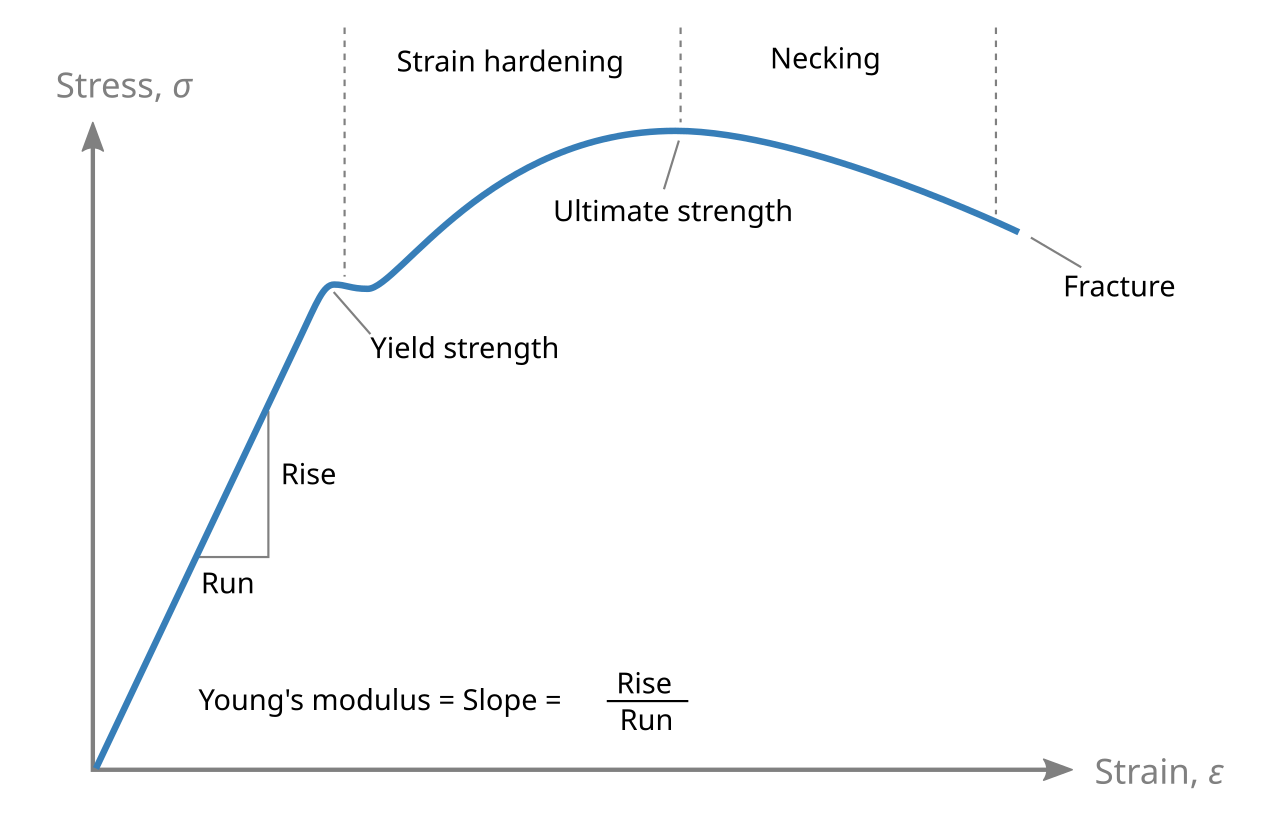
\includegraphics[width=0.8\textwidth]{Stress_Strain_Curve.png}
    \begin{itemize}
        \item \textbf{Modulus of Elasticity ($E$):} Slope in the elastic region.
        \item \textbf{Modulus of Resilience:} Area under the curve up to the yield point, indicating energy absorption before permanent deformation.
        \item \textbf{Modulus of Toughness:} Total area under the curve, representing energy absorption capacity until fracture.
    \end{itemize}
\end{frame}

% Section: Material Ductility and Brittleness
\section{Ductility and Brittleness}
\begin{frame}{Ductility and Brittleness}
    \begin{minipage}[t]{0.45\textwidth}
        \textbf{Ductile Materials:}
        \begin{itemize}
            \item Undergo significant plastic deformation before failure.
            \item Examples include most metals and some polymers.
            \item Ductility measured by percent elongation or reduction in area.
        \end{itemize}
        \vspace{0.5cm}
        \textbf{Brittle Materials:}
        \begin{itemize}
            \item Exhibit little to no plastic deformation before fracture.
            \item Examples include cast iron, glass, and some ceramics.
        \end{itemize}
    \end{minipage}
    \hfill
    \begin{minipage}[t]{0.5\textwidth}
        \vspace{0pt}
        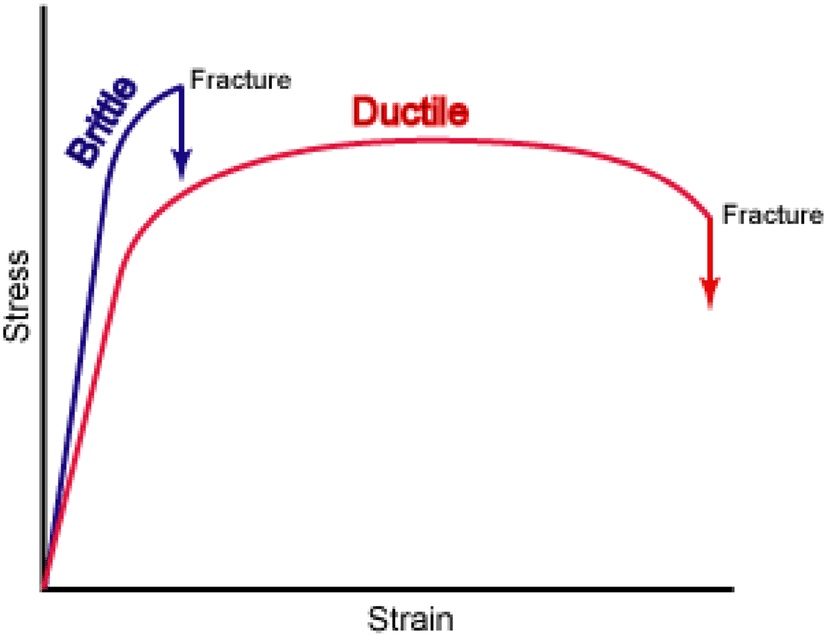
\includegraphics[width=\textwidth]{Ductile_Brittle.png}
    \end{minipage}
\end{frame}

% Section: Strain Energy and Creep
\section{Strain Energy and Creep}
\begin{frame}{Strain Energy and Creep}
    \begin{minipage}[t]{0.49\textwidth}
        \textbf{Strain Energy:}
        \begin{itemize}
            \item Energy stored in a material due to deformation.
            \item \textbf{Modulus of Resilience:} Energy per unit volume up to yield.
            \item \textbf{Modulus of Toughness:} Total energy per unit volume until failure.
        \end{itemize}
        \vspace{0.5cm}
        \textbf{Creep:}
        \begin{itemize}
            \item Gradual deformation under constant stress over time.
            \item Important in high-temperature applications.
        \end{itemize}
    \end{minipage}
    \hfill
    \begin{minipage}[t]{0.45\textwidth}
        \vspace{1pt}
        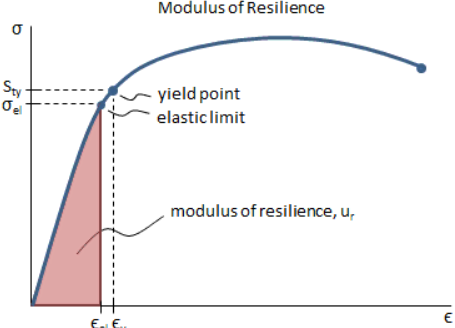
\includegraphics[width=\textwidth]{Creep.png}
        \vspace{2pt}
        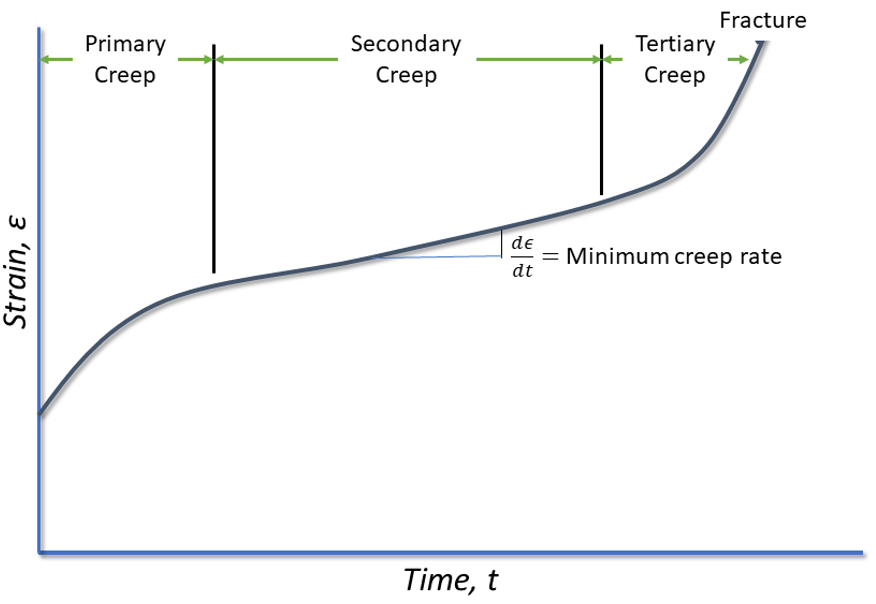
\includegraphics[width=\textwidth]{Creep2.png}
    \end{minipage}
\end{frame}

% Section: Shear Stress and Poisson's Ratio
\section{Shear Stress and Poisson's Ratio}
\begin{frame}{Shear Stress and Poisson's Ratio}
    \begin{minipage}[t]{0.62\textwidth}
        \textbf{Poisson's Ratio ($\nu$):}
        \begin{itemize}
            \item Ratio of lateral strain to longitudinal strain.
            \item Ranges typically from 0 to 0.5 for most materials.
            \item Formula: $\nu = -\frac{\epsilon_{\text{lat}}}{\epsilon_{\text{long}}}$
        \end{itemize}
        
        \textbf{Shear Stress ($\tau$) vs. Shear Strain ($\gamma$):}
        \begin{itemize}
            \item Shear modulus ($G$): $G = \frac{\tau}{\gamma}$
            \item Relationship with Young's modulus: $G = \frac{E}{2(1 + \nu)}$
        \end{itemize}
    \end{minipage}
    \hfill
    \begin{minipage}[t]{0.35\textwidth}
        \vspace{0pt}
        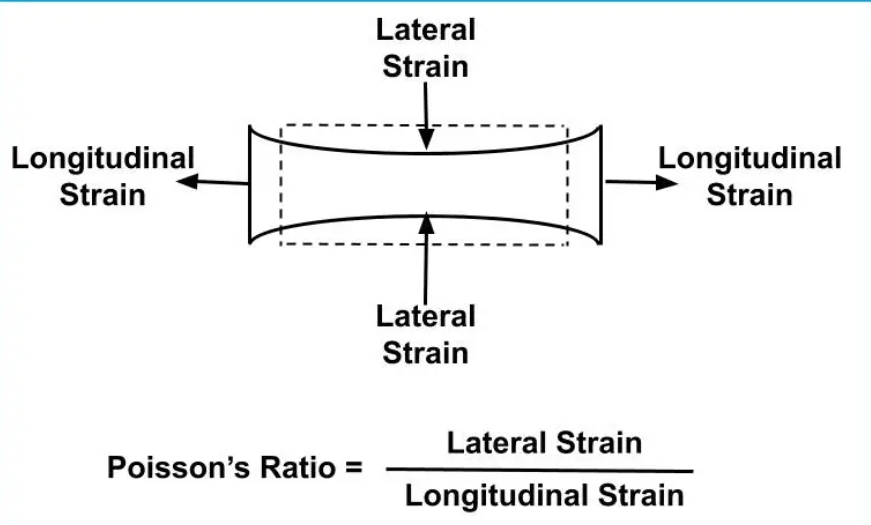
\includegraphics[width=\textwidth]{Ratio.png}
        \vspace{0.2cm}
        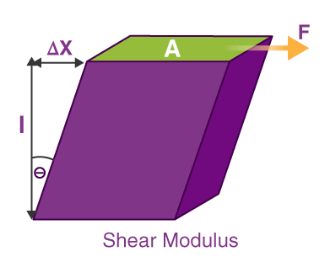
\includegraphics[width=\textwidth]{Shear_Modulous.png}
        \vspace{0.2cm}
        \includegraphics[width=\textwidth]{Shear_Stress.png}
    \end{minipage}
\end{frame}

% Section: Fatigue and Long-term Behavior
\section{Fatigue and Long-term Behavior}
\begin{frame}{Fatigue and Long-term Behavior}
    \begin{minipage}[t]{0.5\textwidth}
        \fontsize{8}{10}\selectfont
        \textbf{Creep:}
        \begin{itemize}
            \item Time-dependent deformation under constant load.
            \item Accelerated by high stress and/or temperature.
            \item Design must ensure materials do not exceed creep limits.
        \end{itemize}
        \vspace{0.2cm}
        \textbf{Fatigue:}
        \begin{itemize}
            \item Failure under repeated loading cycles.
            \item Critical in design to avoid below endurance limit or fatigue strength.
        \end{itemize}
    \end{minipage}
    \hfill
    \begin{minipage}[t]{0.45\textwidth}
        \vspace{0pt}
        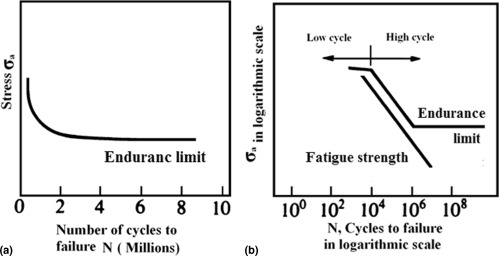
\includegraphics[width=\textwidth]{Fatigue.jpg}
        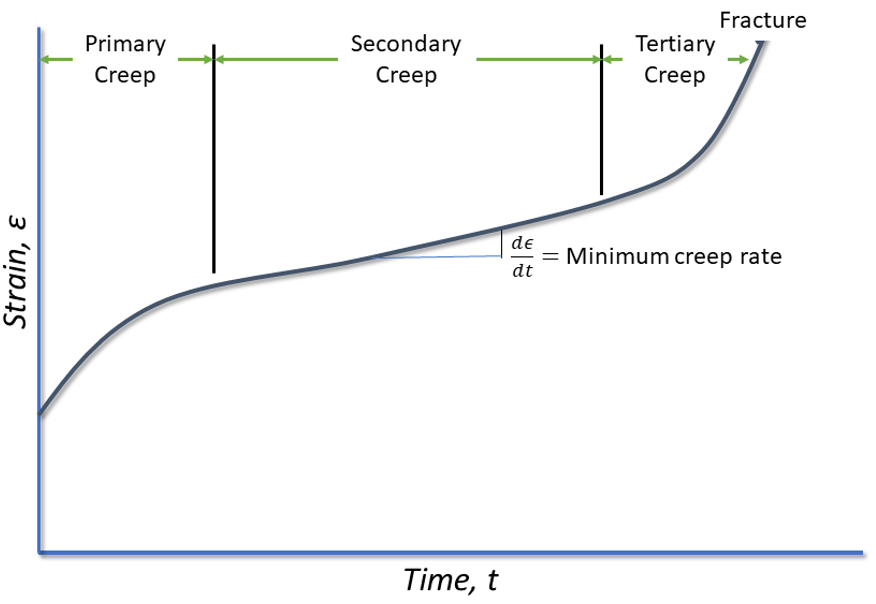
\includegraphics[width=\textwidth]{Creep2.png}
    \end{minipage}
\end{frame}

% Slide: Summary
\section{Summary}
\begin{frame}{Summary}
    \begin{itemize}
        \item Axial loading leads to deformation, crucial for structural integrity.
        \item Thermal stresses must be managed due to temperature changes.
        \item Stress-strain diagrams are key to understanding material behavior.
        \item Strain energy concepts explain material resilience and toughness.
        \item Shear stress and Poisson's ratio affect material response under various loads.
        \item Creep and fatigue are significant for long-term material performance.
    \end{itemize}
\end{frame}

\end{document}



